\documentclass[11pt, oneside]{article} 
\usepackage{geometry}
\geometry{letterpaper} 
\usepackage{graphicx}
	
\usepackage{amssymb}
\usepackage{amsmath}
\usepackage{parskip}
\usepackage{color}
\usepackage{hyperref}

\graphicspath{/Users/telliott_admin/Dropbox/Tex/png/}
% \begin{center} 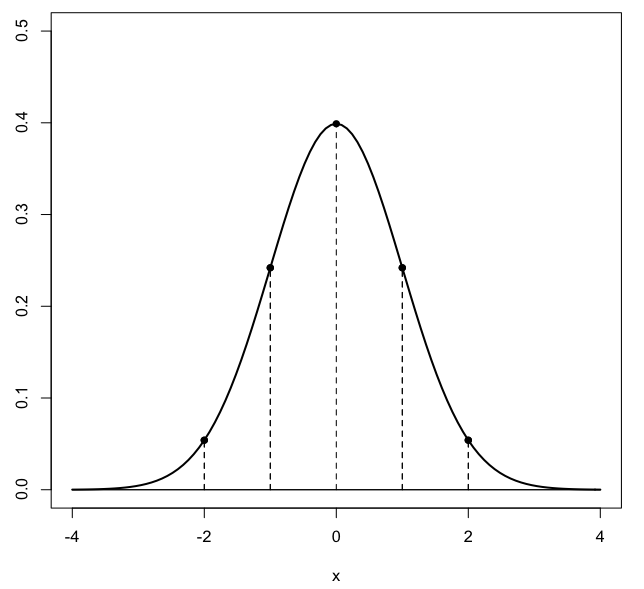
\includegraphics [scale=0.4] {gauss3.png} \end{center}

\title{Galois fields like $GF(2^8)$}
\date{}

\begin{document}
\maketitle
\Large

For cryptography we process bytes (integers in the interval $[0,255]$.  The appropriate Galois field is called GF($2^8$).  We will use cofactors for the polynomials drawn from the set $\{0,1\}$ as before, but we go up to degree 7.

We will use an irreducible polynomial of degree 8 as the modulus.

We closed the last chapter by showing polynomials defined over $GF(2^3)$ modulo the irreducible polynomial $x^3 + x + 1$, which consist of the finite set:
\[ 0 \]
\[ 1 \]
\[ x \]
\[ x + 1 \]
\[ x^2 \]
\[ x^2 + 1 \]
\[ x^2 + x \]
\[ x^2 + x + 1 \]


Kak says:

\begin{quote} Our conceptualization of $GF(2^3)$ is analogous to our conceptualization of the set $Z_8$. The eight elements of $Z_8$ are to be thought of as integers modulo 8. So, basically, $Z_8$ maps all integers to the eight numbers in the set $Z_8$. Similarly, $GF(2^3)$maps all of the polynomials over $GF(2)$ to the eight polynomials shown above.\end{quote}

He continues:

\begin{quote}$GF(2^3)$ contains a unique multiplicative inverse for every non- zero element for the same reason that $Z_7$ contains a unique multiplicative inverse for every non-zero integer in the set. (For a counterexample, recall that $Z_8$ does not possess multiplicative inverses for 2, 4, and 6.) 

Stated formally, we say that for every non-zero element $a \in$ $GF(2^3)$ there is always a unique element $b \in$ $GF(2^3)$ such that $a \times b = 1$.

The above conclusion follows from the fact if you multiply a non-zero element $a$ with each of the eight elements of $GF(2^3)$, the result will be the eight distinct elements of $GF(2^3)$. 

Obviously, the results of such multiplications must equal 1 for exactly one of the non-zero elements of $GF(2^3)$. So if $a \times b = 1$, then $b$ must be the multiplicative inverse for $a$.

The same thing happens in $Z_7$. If you multiply a non-zero element $a$ of this set with each of the seven elements of $Z_7$, you will get seven distinct answers. The answer must therefore equal $1$ for at least one such multiplication. When the answer is $1$, you have your multiplicative inverse for $a$.\end{quote}.

In fact

\begin{quote}For a more formal proof (by contradiction) of the fact that if you multiply a non-zero element a of $GF(2^3)$ with every element of the same set, no two answers will be the same, let's assume that this assertion is false. That is, we assume the existence of two distinct values $b$ and $c$ in the set such that \end{quote}

\[ a \times b \equiv a \times c \mod (x^3 + x + 1) \]
which implies
\[ a \times (b - c) \equiv 0 \mod (x^3 + x + 1) \]
which implies either $a = 0$ or $b = c$, in either case this is a contradiction.

In exploring multiplication in $GF(2^8)$ constructed with the irreducible polynomial
\[ x^8 + x^4 + x^3 + x + 1 \]

My approach was to show by exhaustive search that every number has a unique multiplicative inverse, and furthermore for every product other than $1$ and every factor $a$ there is a unique $b$ such that $a \times b = p$.  We'll get to this later.

\subsection*{addition}

The fundamental definition of addition for our Galois field $GF(2^8)$  is that it is the same as the XOR operation:
\[ a \oplus b \]

Since $a \oplus a = 0$, it follows that each number is its own additive inverse, with a + a = 0.  Addition is the same as subtraction.  

And from this a clear implication is that multiplication is \emph{not} repeated addition.

The irreducible polynomial that is used for $GF(2^8)$ is
\[ x^8 + x^4 + x^3 + x + 1 \]

It is claimed that the finite field $GF(2^8)$ contains 256 distinct polynomials over $GF(2)$.

\subsection*{representations}

A common way to write numbers in $GF(2^8)$ is like this
\[ = x^7 + x^6 + x^5 + x^2 + x^1 + x^0 \]
the exponents on the last two terms are typically suppressed:
\[ =  x^7 + x^6 + x^5 + x^2 + x + 1 \]

If a term is present, then a $1$ is present in the place corresponding to the exponent, counting from right to left and starting with index 0. So

\[ x^7 + x^6 + x^5 + x^2 + x + 1 \]

is the same as binary $1110 \  \  0111$ or \textbf{0xe7}.  In fact, exactly the integers 0-255 or hex \textbf{00} to \textbf{ff} are in this field.

\subsection*{multiplication}

Multiplication by 1 is the easiest:  $b * 1 = b$, which is a great relief.

Multiplication by any number $\ge 2$ consists of two steps:  the multiplication itself, possibly followed by a mod operation.

\subsection*{multiplication by 2}

For multiplication by 2 there are two cases:  if the most significant bit (MSB) of $b$ is not set ($b \le 127$) then we simply do a left-shift:  throw away the left-hand 0 bit from $b$ and insert a $0$ bit on the right
\[ 0111 \  \  1111 * 2 =  1111 \  \  1110 = b' \]

If $b$ \emph{does} have its most-significant bit set ($b > 127$), first do the shift (and throw away the bit in the $x^8$ place).  Then do the mod operation, which can be achieved by XOR with 27 ($ = 0001\ 1011$)	:
\[ b' \oplus 27 \]

We can carry out higher multiplication as successive multiplications and XOR by powers of two.  The procedure above carries out XOR every time the product exceeds 256 (and since we're multiplying by 2 it can't exceed 512),  So, we never need to worry about products larger than 512.

\subsection*{multiplication by powers of 2}

To multiply by 4 simply carry out two successive multiplications by 2.
\[ b * 4 = (b * 2) * 2 \]

For higher powers, lather, rinse and repeat:

\[ b * 8 = (b * 4) * 2 = ((b * 2) * 2) * 2 \]

\subsection*{multiplication by any number in GF($2^8$)}
Suppose we want to multiply $ 1000 \  \  0011 * b$.  First use the distributive law to write
\[ 1000 \   0011 * b \]
\[ = \ [ \ 1000 \   0000  + 0000 \  0010  + 0000 \   0001 \ ] \ * b \]
\[ = 1000 \  0000 * b + 0000 \  0010 * b + 0000 \  0001 * b \]
Break the multiplier into its constituent powers of two, multiply as before, and then carry out a final  addition step (which is just $\oplus$).

And that is really all we need.

When you get into the mechanics of AES, you 'll find that multiplying a 4-byte sequence like \textbf{db 13 53 45} by the matrix below to yield \textbf{8e 4d a1 bc} 

\[ fM =
\begin{bmatrix}
2 & 3 & 1 & 1 \\
1 & 2 & 3 & 1 \\
1 & 1 & 2 & 3 \\
3 & 1 & 1 & 2
\end{bmatrix} 
*
\begin{bmatrix}
db \\
13 \\
53 \\
45
\end{bmatrix} 
=
\begin{bmatrix}
8e \\
4d \\
a1 \\
bc
\end{bmatrix} 
\]

is reversed by multiplying the latter by

\[ rM = 
\begin{bmatrix}
14 &11 &13 & 9 \\
9 &14 &11 & 13 \\
13 & 9 &14 & 11 \\
11 &13 & 9 & 14
\end{bmatrix} \]

The reason is that 
\[ fM \times fM \times fM = rM \]
and
\[ fM \times fM \times fM \times fM \]
\[ = fM \times rM = I \]

Which means that
\[ rM \times (fM \times \mathbf{A}) \]
\[ = ( rM \times fM) \times \mathbf{A} \]
\[ =I \mathbf{A} =  \mathbf{A} \]

\end{document}